%==========================================================================
% Capítulo 1: O que é LaTeX?
%==========================================================================
\chapter{O que é \LaTeXX} 
\label{cap:LaTeX}

Esse capítulo é um pouco polêmico!
Alguns provavelmente falarão que não precisaria abordae tais tópicos em um 
minicurso de 3\unit{h}, vist que poderíamos ser mais diretos e realizarmos 
logo a prática. 
Entretanto, entendo que é um tópico importante, que definirá algumas ideias 
sobre o que é o \LaTeXX, bem como se propõe a uma abordagem mais atual dos 
recursos disponibilizados para composição tipográfica. 
Penso que, se eu soubesse dessas coisas logo na minha iniciação no \LaTeXX, 
teria uma visão bem mais consistente de seu uso. 

% seção 01 ================================================================

\section{Como se fala \LaTeXX?}
\label{sec:como-se-fala}

Pode até ser irrelevante essa informação, mas é sempre bom conhecermos as 
coisas corretamente, não? 

Sei que vocês sabem que não estamos falando daquela seiva da árvore que é 
usada para produzir diferentes materiais como tinta, luvas, etc. 
Ou seja, não estamos falando do Látex. 

O \LaTeXX\ não é Látex. 
Nem na ideia, nem na pronúncia. 

Existem duas maneiras aceitáveis para pronunciar o nome em questão: uma mais
voltada ao inglês e outra mais ``abrasileirada''. 

Antes de exibir a pronúncia, entretando, vamos conhecer a pronúncia da 
palavra \TeX.
Não é \textit{Téckis}, mas \textit{Téc} (como em ``\textbf{tec}nologia''). 
Isso se deve ao fato de que a palavra \TeX, na realidade, veio da junção 
das três letras gregas: {\grega τ} (tau);\, {\grega ε} (épsilon); e, 
{\grega χ} (chi --- lê-se \textit{Qui}, como em ``\textbf{Qui}abo'').
Essas letras gregas, juntas e em maiúsculas, ficam: {\grega ΤΕΧ}; mas o 
idealizador dessa linguagem de programação, como veremos, denominada \TeX, 
simplesmente quis modificar a disposição do {\grega Ε} para mostrar que se 
trata de algo relacionado à tipografia.

A tipografia é a arte e o processo de criação na composição e impressão de um 
texto, física ou digitalmente (Wikpédia).

É interessante notarmos que a palavra \TeX\ está relacionada à 
\textsf{tecnologia}, visto que é uma linguagem de programação; mas também 
relacionada à \textsf{arte}, visto que a tipografia é descentende da 
\textit{Caligrafia} --- uma arte que resiste ao tempo e traça muitos parâmetros para formas elegantes de letras/fontes.
Isso não é ao acaso!
A palavra \TeX\ foi escolhida justamente porque as palavras \textsf{arte} 
({\grega τεχνη}) e \textsf{tecnologia} ({\grega τεχνολογία}) possuem a mesma raiz linguística {\grega τεχ}. 

Do exposto, agora podemos indicar as formas aceitáveis de pronunciar a palavra\LaTeXX.

\begin{itemize}
  \item[\emoji{speaking-head}] Se você quiser pronunciar mais parecido com o        Inglês, fale ``\textit{LeiTéc}''. 
  \item[\emoji{speaking-head}] Mas, se quiser falar mais abrasileirado, use 
        ``\textit{LaTéc}''.
  \item[\emoji{prohibited}] Apenas, evite, depois desse minicurso, falar 
        ``\textit{LaTéckis}''; ou, pior ainda, ``\textit{LáTeckis}''. \emoji{winking-face-with-tongue}
\end{itemize}

% seção 02: Mas, o que é o LaTeX ==========================================

\section{Já sei falar, mas o que é \LaTeXX?}
\label{sec:word-latex}

Tudo bem\ldots\
Como vocês já sabem pronunciar corretamente a essa palavra, vamos agora
dizer \ldots\ o que \textbf{não} é \LaTeXX. 

Calma, mas alguns, no início, costumam comparar o \LaTeXX\ com algum editor 
de textos, como o Word ou LibreOffice. 
O \LaTeXX\ não é um editor de textos!
E, mesmo que fôssemos comparar, a filosofia seria diferente!
Editores como Word ou LibreOffice são \textsf{WYSIYYG} (\textit{What You See Is What You Get} --- O que você vê é o que você tem); ou seja, se você 
quer um símbolo como $\sum$, você precisa clicar sobre ele em algum lugar
do editor.
Na filosofia do \LaTeXX, você digita comandos e depois é necessário uma 
\textit{compilação}, para que os símbolos (e o próprio texto) sejam 
exibidos adequadamente.

Então, já temos uma ideia do que \textbf{não} é o \LaTeXX!
Não é um editor de textos!
E, por conta disso, é natural que curva de aprendizado seja um pouco 
diferente: é necessário uma aquisição prévia de vocabulários para comandos. 
Entretanto, espera-se uma flexibilidade e otimização de tarefas tipográficas
à medida que esse vocabulário é expandido, principalmente quando o texto 
que se deseja produzir é complexo (com \textit{hiperlinks}; referências 
cruzadas; referências bibliográficas; index; muitas figuras ou tabelas; 
etc.). 
Veja a Figura~\ref{fig:latex-vs-word} para essa comparação hipotética. 

\begin{figure}[!htbp]
  \centering
    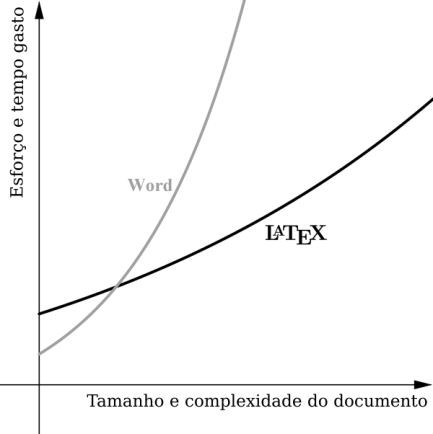
\includegraphics[width=0.7\textwidth]{latex-vs-word}
  \caption{Curva de aprendizado}
  \label{fig:latex-vs-word}
\end{figure}

Vocês estão percebendo que o \LaTeXX\ está parecendo uma espécie de 
\textsf{linguagem}, visto que há uma aquisição de vocabulário, estruturas 
e organização. 
Mas, que tipo de ``linguagem'' seria o \LaTeXX?

% subsection 03: TeX vs LaTeX ---------------------------------------------

\subsection{\TeX\ vs \LaTeXX}
\label{subsec:tex-latex}

Para entender que tipo de linguagem é o \LaTeXX, precisamos conhecer o que 
é o \TeX. 

Tudo começou quando 
\href
{
  https://en.wikipedia.org/wiki/Donald_Knuth
}
{
  \sffamily
  Donald Ervin Knuth
}
recebeu uma cópia de seu novo livro de programação. 
Ele simplesmente não se conformou com o resultado tipográfico em suas mãos. 
Como cientista da computação Knuth pensou que poderia criar uma linguagem 
de programação que preenchesse harmoniosamente, com algum algorítmo 
engenhoso, com o ``0'' (zero), para espaços onde \textbf{não há} ``tinta'';
e, ``1'' (um) para espaços \textbf{com} tinta.
Foi formada a idea do \TeX, no final dos anos 70. 

A linguagem \TeX\ produzia comandos primitivos essenciais, mas 
ainda era preciso criar um conjunto de ``atalhos'' (macros) para certas 
estruturas de um texto, por exemplo. 
O próprio Knuth produziu esse conjunto de macros, inicialmente, denominado 
\textsf{Plain \TeX}.
Mas, ao que parece, esse conjunto de macros ainda dava muito trabalho para 
ser usado! \emoji{sweat-smile}

Foi, então, que, em 1985, Lamport criou um conjunto de macros muito especial: \LaTeXX. 
Inclusive, o ``{\grega La}'' de \LaTeXX, veio do ``La'' de Lamport.
Esse conjunto de macros facilita nossa vida até hoje!
Lembrem-se disso: 

\tcboxC{
  \sffamily
  O \LaTeXX\ veio para facilitar nossa vida!
}


Entretando, não nos enganemos: o \LaTeXX\ não é uma simples linguagem de 
marcação! 
Ele é um sistema de preparação de documentos, em alta qualidade tipográfica.

% Seção 03: Onde posso encontrar o LaTeX? ---------------------------------- 

\section{Onde posso encontrar o \LaTeXX?} 
\label{sec:encontrar}

Quando geralmente falamos ``Quero instalar o \LaTeXX\ em meu computador'', na 
realidade estamos instalando programas de uma \textbs{Distribuição} do \LaTeXX. 

Cada distribuição tem sua característica, mas, geralmente, selecionam um 
conjunto de: 
\begin{itemize}
  \item \textis{Fontes}. Quer textual (serifada, sem serifa, monoespaçada, etc.), 
        quer matemática (para expressões matemáticas); 
  \item \textis{Pacotes}. Falaremos sobre alguns deles depois, todavia, por hora, 
        basta sabermos que são implementações de funcionalidades diversas no 
        \LaTeXX: desde simples notações convenientes em certos contextos, até 
        estruturas mais complexas em cabeçalhos estilizados ou desenhos; 
  \item \textis{Editores}. Usados para facilitar a escrita do código em \LaTeXX.
        Em geral, os editores que já estão disponíveis numa distribuição, são 
        bem básicos. 
        TeXworks é um exemplo de editor de texto para \LaTeXX\ que vem em algumas 
        distribuições; 
  \item \textis{Interpretadores}. Também chamados de \textis{engines}. 
        Aqui é o coração do \LaTeXX: eles é que são responsáveis por transformar 
        o que digitamos, em algum formato para visualização (que hoje, 
        predominantemente, é o \texttt{pdf})
  \item \textis{Compiladores}. Se os Interpretadores são o coração do \LaTeXX, 
        os compiladores são o sangue. 
        São com eles que nos cominicamos e eles se comunicam com os Interpretadores. 
        Exitem algumas opções, mas vou destacar três: 
        \begin{enumerate}
          \item \texttt{pdflatex}: o mais tradicional. 
                Geralmente vem como padrão na maioria das distribuições. 
                Ele usa o interpretador \hologo{pdfTeX} para produzir a saída 
                em \texttt{pdf}, do código escrito em \LaTeXX. 
          \item \texttt{lualatex}: sucessor oficial do \texttt{pdflatex}. 
                A nova versão do \LaTeXX, denominada \hologo{LaTeX3}, usará, por 
                padrão, o \hologo{LuaTeX} como \textit{engine}; e, por conseguinte, 
                o \texttt{lualatex} será o \textit{compilador} principal.  
                \begin{itemize}
                  \item[\emoji{warning}] Em nosso minicurso, já usaremos o 
                         \texttt{lualatex} para compilação. 
                \end{itemize}
          \item \texttt{xelatex}: usa o \hologo{XeTeX} como \textit{engine}. 
                É um pouco mais antigo que o \texttt{lualatex}, e possui 
                funcionalidades semelhantes (como possibilidade de escolher  
                fontes do próprio sistema -- coisa que o \hologo{pdfTeX} não faz), 
                embora já esteja bem mais maduro em muitos pontos.
                Mas, como o \hologo{LuaTeX} é escrito em Lua (uma linguagem de 
                programação bem otimizada e em ascenção), a tendendia é alcançar 
                muito mais funcionalidades, com flexibilidade; além dos 
                desenvolvedores de pacotes implementarem tais funcionalidades 
                primeiro em Lua. 
        \end{enumerate}
  \item \textis{Ferramentas diversas}. Por exemplo, ferramentas de automação. 
        Muitas vezes, quando a complexidade do documento exige, precisamos fazer 
        mais de uma compilação. 
        Existem ferramentas que auxiliam nesse sentido. 
        Uma delas é o \texttt{latexmk}, que busca no arquivo \texttt{.log} (
        gerado na compilação) o que é necessário para uma compilação completa. 
        Acaba sendo meio ``mágico'' e você não tem muito controle sobre isso. 
        Caso queira mais controle nesse processo de automação na compilação, uma 
        alternativa é o {\arara arara}. 
        Nele, estabelecemos diretrizes (através de comentários especiais no 
        início do código) para a compilação completa de nosso texto. 
        Falaremos mais sobre essas ferramentas no Apêndice~\ref{app:arara}
\end{itemize}

Existem muitas distribuições do \LaTeXX, mas destaco as seguintes:

\begin{itemize}
  \item \href{https://miktex.org/}{\textsf{MiK\TeX}}. 
        É uma distribuição multiplataforma, ou seja, pode ser 
        seus programas podem ser instalados em sistemas como Linux\footnote{
          obviamente aqui não estou tratando apenas no \textit{kernel}; mas, 
          dele; dos programas GNU; e de outros programas fora do GNU
        }; Windows ou MacOS. 
        Um diferencial dessa distribuição é a possibilidade de instalar um 
        conjunto de pacotes básicos e, à medida que você for precisando de mais 
        pacotes, a instalação é automática. 
  \item \href{https://www.tug.org/texlive/}{\textsf{\TeX Live}}. 
        Tradicional distribuição para sistemas Linux, mas 
        também é multiplataforma. 
        Você pode instalar a versão \textit{full}, ou seja, com todos os pacotes 
        disponíveis, ou algumas variações, sendo que é necessário instação manual 
        de futuros pacotes, caso necessário. 
  \item \href{https://www.tug.org/mactex/}{\textsf{Mac \TeX}}. 
        Distribuição voltada, exclusivamente, para sistemas MacOS.
\end{itemize}

A Figura~\ref{fig:distro} sintetiza essas explanações sobre distribuições. 

\begin{figure}[!htbp]
  \centering
    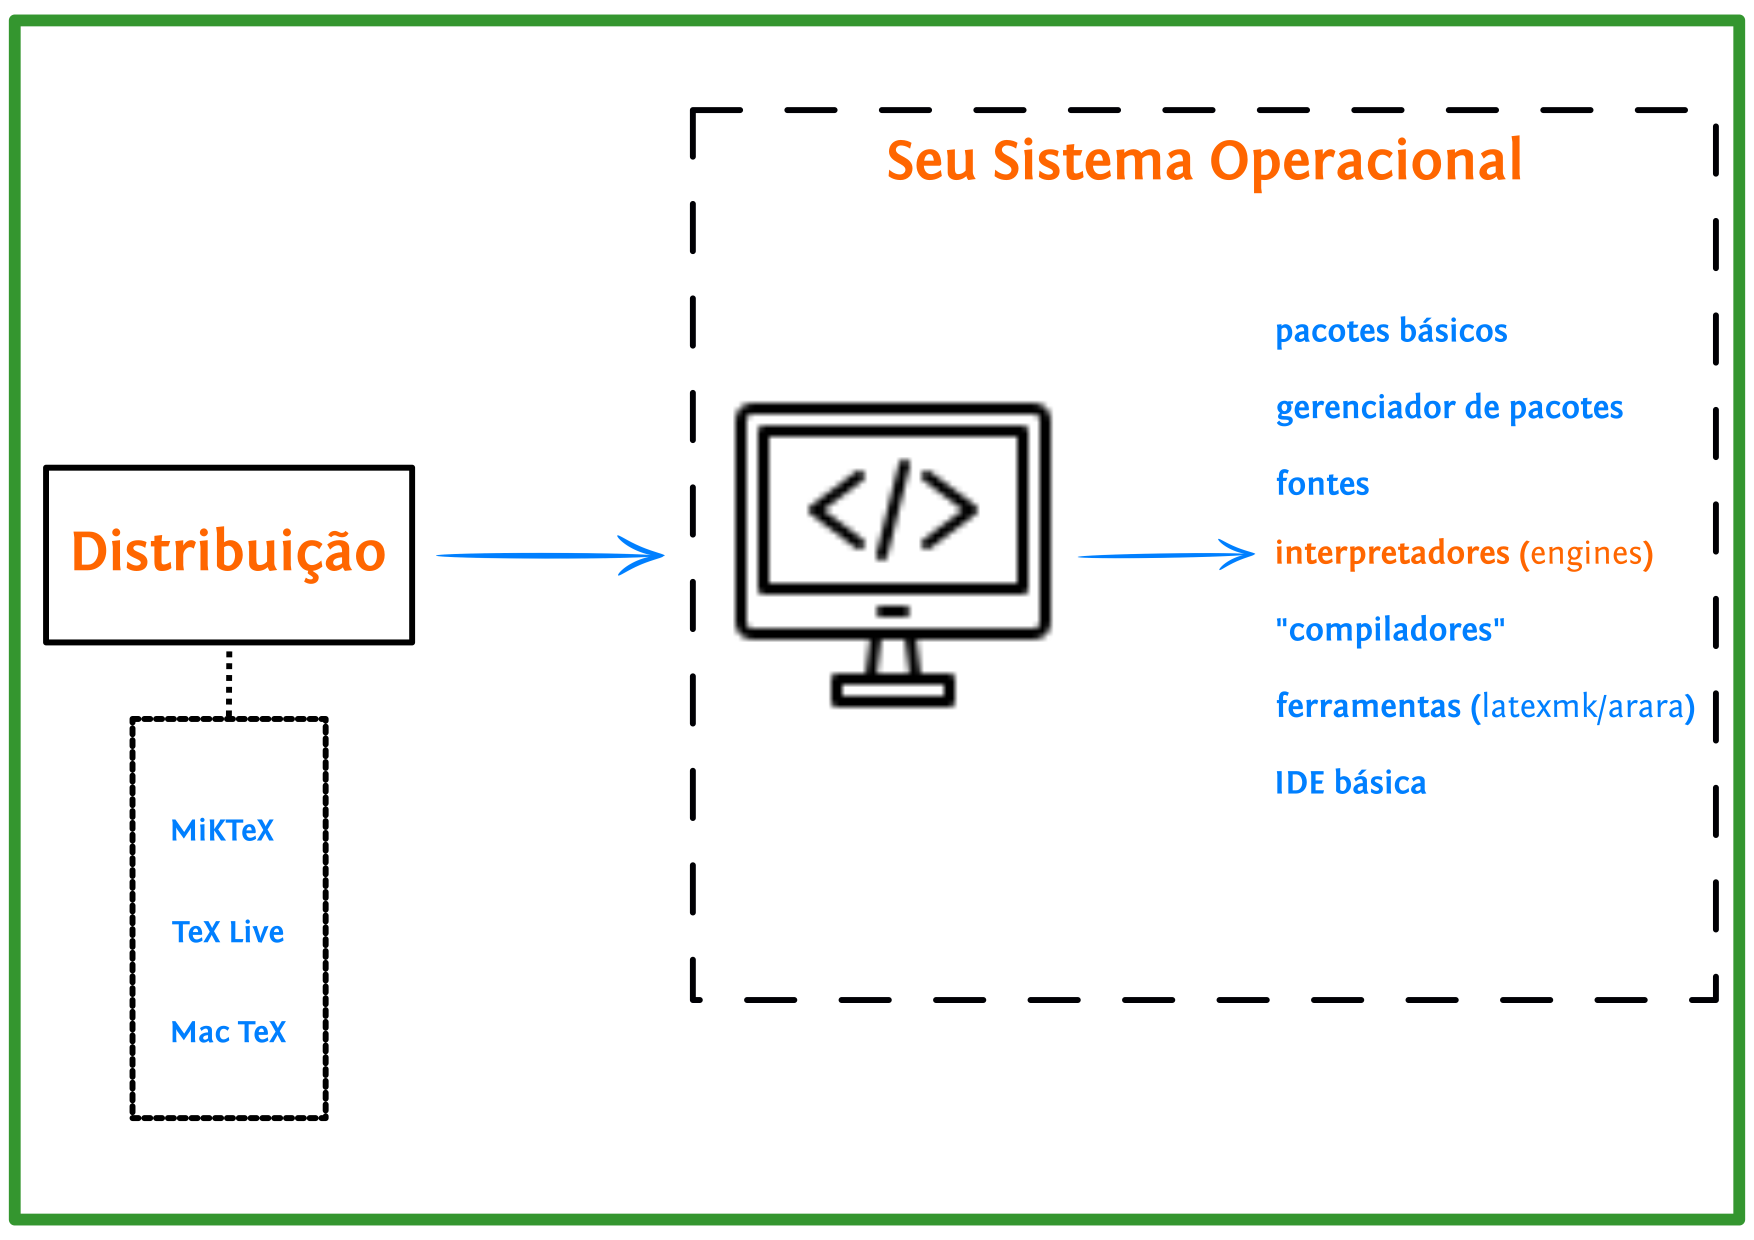
\includegraphics[width=0.95\textwidth]{distro.png}
  \caption{Distribuições e o que geralmente oferencem para instalação}
  \label{fig:distro}
\end{figure}

\subsection{Versões do \LaTeXX} %-------------------------------------------

Mais uma vez vamos falar sobre nomes\ldots \emoji{hand-over-mouth}

Quando falamos ``\LaTeXX'', já vimos que não estamos tratando de Editores de 
Texto; seiva de árvores; etc., mas de uma linguagem. 
Ok!
Mas, você sabe que linguas mudam, certo?
Com o \LaTeXX\ não seria diferente! 

A versão atual (também chamada de \textit{release}) é a 
{\grega \hologo{LaTeX2e}}; que foi sucessora da versão anterior a 1994, a saber, 
{\grega \LaTeX 2.09}. 

Assim, quando falamos ``\LaTeXX'', na realidade estamos evocando o {\grega \hologo{LaTeX2e}}. 

Além disso, há um projeto de longo prazo para uma profunda reconfiguração do 
\LaTeXX: o {\grega \LaTeX 3}. 

\begin{figure}[!htbp]
  \centering
    
\includegraphics[width=0.95\textwidth]{latex-project-logo.png}
  \caption{\href{https://www.latex-project.org/latex3/}{https://www.latex-project.org/latex3/}}
\end{figure}

Continuaremos a falar \LaTeXX, mas não se esqueça que estamos na \textit{release} 
{\grega \hologo{LaTeX2e}}. 

Se você quiser saber mais sobre as diferentes versões, dê uma olhada aqui: 

\begin{center}
  \footnotesize
  \url{https://www.latex-project.org/news/latex2e-news/ltnews.pdf}
\end{center}

Em resumo poderíamos dizer: 
Uma \textis{Distibuição} fornece um \textis{Formato} (\textit{format} --- no 
nosso caso, \hologo{LaTeX2e}; mas, exitem outros, como por exemplo 
\hologo{ConTeXt}); um conjunto de \textis{compiladores} (\hologo{pdfTeX}, 
\hologo{LuaTeX}, \hologo{XeTeX}) e \textis{interpretadores} ({\grega\hologo{pdfLaTeX}}, 
{\grega\hologo{LuaLaTeX}}, {\grega \hologo{XeLaTeX}}); além de \textit{fontes}, 
\textit{pacotes básicos} e \textit{ferramentas} que auxiliam a composição 
tipográfica. 

\subsection{Algo sobre Editores} %------------------------------------------

Certamente você pode escrever seu texto, em \LaTeXX, num editor de textos de 
sua preferência! 
Inclusive num ``bloco de notas'', ou num ``gedit'' da vida. 
Mas, certamente há editores mais convenientes, não?
Aliás, podemos ir além de editores e considerarmos verdadeiros IDE (
\textit{Integrated Development Environment} --- Ambiente de Desenvolvimento Integrado ).

Exitem editores mais gerais e outros específicos para escrita de cógido em 
\LaTeXX. 

No que se refere aos editores gerais, realmente existem muitos:
\href{https://neovim.io/}{Neovim};
\href{https://code.visualstudio.com/}{VSCode};
\href{https://www.gnu.org/software/emacs/}{GNU Emacs};
\href{https://www.sublimetext.com/}{Sublime Text}; 
\href{https://atom.io/}{Atom};
\href{https://www.geany.org/}{Geany};
etc.

Particularmente, já usei o VSCode e o Neovim.
No VSCode, deve-se instalar um \textit{plugin} específico (LaTeX Workshop) para 
funcionalidades de autocompletar, compilação, etc.
Se você quiser usar algum interpretador diferente do \hologo{pdfTeX}, é 
necessário configurar manualmente. 
Já o Neovim, é um editor que deriva do Vim (um excelente editor de textos), que 
possui como uma de suas ``filosofias'' não retirar a mão do teclado para 
codificar, ou seja, evitar o contato com o \textit{mouse} (o que pode ajudar em 
certas dores no braço). 
Precisa de muitas configurações prévias e pode ser desafiador no início, mas 
você pode deixá-lo do seu jeito, por sua flexibilidade. 
Falando em flexibilidade, ele é escrito em Lua e o desenvolvimento de 
\textit{plugins} está em plena ebulição. 

Obviamente, para quem está começando no \LaTeXX, aconselha-se editores 
dedicados (ou específicos); pois a configuração é mínima para iniciar o 
processo de escrita e compilação (composição tipográfica).
Você pode comparar uma lista generosa deles no \textit{link}:

\begin{center}
  \footnotesize
  \url{https://en.wikipedia.org/wiki/Comparison_of_TeX_editors}
\end{center}

Em especial, destaco o \href{https://www.texniccenter.org/}{\TeX nicCenter}, 
para quem é usuário de Windows; ou o 
\href{https://www.texstudio.org/}{\TeX studio}, que é multiplataforma. 

\begin{atencao}{Atenção!}{\exclamacao} 
  Para esse minicurso, usaremos o \href{https://pt.overleaf.com/}{\textsf{Overleaf}}. 
  Ele é um editor de \LaTeXX online com muitas vantagens para o formato de nosso 
  minicurso: sem instalação; possibilidade de colaboração em tempo real; 
  possibilidade de controle de versões; centenas de templates disponíveis; etc. 
  Escolhi fazer no \textsf{Overleaf}; pois, não precisarei me preocupar com erros 
  comuns de instação; além de proporcionar uma visualização do resuldado quase 
  em tempo real. 
  É necessário cadastro (pode usar uma conta \textsf{Google} também) na plataforma. 
  Não se preocupem que ainda é gratuito. 
  O Apêndice~\ref{app:overleaf} trará mais informações! 
\end{atencao}
